\documentclass[aspectratio=169, 10pt]{beamer}

% ── Theme & Colors ──────────────────────────────────────────────────
\usetheme{Madrid}
\usecolortheme{whale}
\definecolor{darkblue}{RGB}{0,51,102}
\definecolor{lightblue}{RGB}{230,240,250}
\definecolor{accentorange}{RGB}{230,120,30}
\definecolor{accentgreen}{RGB}{34,139,34}
\definecolor{accentred}{RGB}{200,50,50}
\setbeamercolor{title}{fg=white,bg=darkblue}
\setbeamercolor{frametitle}{fg=white,bg=darkblue}
\setbeamercolor{block title}{fg=white,bg=darkblue}
\setbeamercolor{block body}{bg=lightblue}
\setbeamercolor{block title alerted}{fg=white,bg=accentred}
\setbeamercolor{block body alerted}{bg=accentred!8}
\setbeamercolor{block title example}{fg=white,bg=accentgreen!80!black}
\setbeamercolor{block body example}{bg=accentgreen!8}
\setbeamercolor{item}{fg=darkblue}
\setbeamercolor{structure}{fg=darkblue}
\setbeamertemplate{navigation symbols}{}
\setbeamertemplate{footline}{%
  \leavevmode%
  \hbox{%
    \begin{beamercolorbox}[wd=.33\paperwidth,ht=2.5ex,dp=1ex,center]{author in head/foot}%
      \usebeamerfont{author in head/foot}\insertshortauthor
    \end{beamercolorbox}%
    \begin{beamercolorbox}[wd=.34\paperwidth,ht=2.5ex,dp=1ex,center]{title in head/foot}%
      \usebeamerfont{title in head/foot}\insertshorttitle
    \end{beamercolorbox}%
    \begin{beamercolorbox}[wd=.33\paperwidth,ht=2.5ex,dp=1ex,right]{date in head/foot}%
      \usebeamerfont{date in head/foot}\insertframenumber{} / \inserttotalframenumber\hspace*{2ex}
    \end{beamercolorbox}}%
  \vskip0pt%
}

% ── Packages ────────────────────────────────────────────────────────
\usepackage{amsmath,amssymb,bm}
\usepackage{booktabs}
\usepackage{tikz}
\usetikzlibrary{arrows.meta,positioning,shapes.geometric,calc,fit,decorations.pathreplacing,backgrounds}
\usepackage{pgfplots}
\pgfplotsset{compat=1.18}
\usepackage{array}
\usepackage{multirow}
\usepackage{mathtools}

% ── Shortcuts ──
\newcommand{\R}{\mathbb{R}}
\newcommand{\Loss}{\mathcal{L}}
\newcommand{\vect}[1]{\bm{#1}}
\newcommand{\mat}[1]{\mathbf{#1}}
\DeclareMathOperator{\ReLU}{ReLU}
\DeclareMathOperator{\LN}{LayerNorm}

% ── Meta ──
\title[LSGNN-DualTask]{LSGNN-DualTask}
\subtitle{A Graph Neural Network with Edge Consistency Regularization\\for Network Intrusion Detection}
\author[Authors]{Author One \and Author Two \and Author Three}
\institute[University]{Department of Computer Science \\ University Placeholder}
\date{2025--2026}

\begin{document}

% ═══════════════════════════════════════════════════════════════════
% SLIDE 1 — Title
% ═══════════════════════════════════════════════════════════════════
\begin{frame}
\titlepage
\end{frame}

% ═══════════════════════════════════════════════════════════════════
% SLIDE 2 — Outline
% ═══════════════════════════════════════════════════════════════════
\begin{frame}{Outline}
\tableofcontents
\end{frame}

% ═══════════════════════════════════════════════════════════════════
\section{Introduction \& Motivation}
% ═══════════════════════════════════════════════════════════════════

% SLIDE 3 — Problem Statement
\begin{frame}{Network Intrusion Detection: The Challenge}
\begin{columns}[T]
\begin{column}{0.55\textwidth}
\begin{block}{Problem}
Detect malicious activities in network traffic \textbf{in real time}
\end{block}
\vspace{0.3cm}
\textbf{Traditional approaches:}
\begin{itemize}
    \item Signature-based matching --- \textit{cannot detect novel attacks}
    \item Statistical thresholds --- \textit{high false positive rate}
    \item ML on flat features --- \textit{ignores relational structure}
\end{itemize}
\vspace{0.3cm}
\textbf{Key insight:} Network traffic is inherently \textbf{relational} --- flows between hosts form a \textbf{graph structure}.
\end{column}
\begin{column}{0.42\textwidth}
\centering
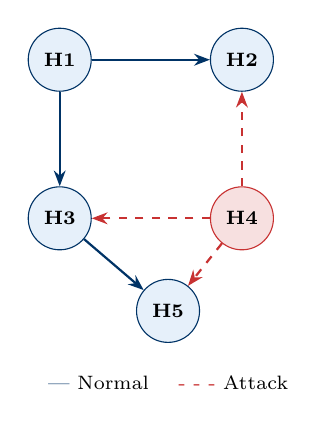
\begin{tikzpicture}[
    host/.style={circle, draw=darkblue, fill=lightblue, minimum size=0.8cm, font=\scriptsize\bfseries},
    attack/.style={circle, draw=accentred, fill=accentred!15, minimum size=0.8cm, font=\scriptsize\bfseries},
    flow/.style={-{Stealth[length=2mm]}, thick},
    badflow/.style={-{Stealth[length=2mm]}, thick, color=accentred, dashed}
]
    \node[host] (h1) {H1};
    \node[host, right=1.5cm of h1] (h2) {H2};
    \node[host, below=1.2cm of h1] (h3) {H3};
    \node[attack, below=1.2cm of h2] (h4) {H4};
    \node[host, below right=0.6cm and 0.8cm of h3] (h5) {H5};

    \draw[flow, darkblue] (h1) -- (h2);
    \draw[flow, darkblue] (h1) -- (h3);
    \draw[flow, darkblue] (h3) -- (h5);
    \draw[badflow] (h4) -- (h2);
    \draw[badflow] (h4) -- (h3);
    \draw[badflow] (h4) -- (h5);

    \node[below=0.3cm of h5, font=\scriptsize] {{\color{darkblue}---} Normal \quad {\color{accentred}- - -} Attack};
\end{tikzpicture}
\end{column}
\end{columns}
\end{frame}

% SLIDE 4 — Three Challenges
\begin{frame}{Three Key Challenges}
\begin{columns}[T]
\begin{column}{0.32\textwidth}
\begin{block}{\centering Sparse Features}
\centering
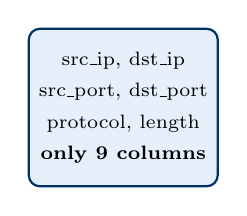
\begin{tikzpicture}[scale=0.8]
    \draw[fill=lightblue, draw=darkblue, thick, rounded corners] (0,0) rectangle (3,2.5);
    \node[font=\scriptsize, align=center] at (1.5,2) {src\_ip, dst\_ip};
    \node[font=\scriptsize, align=center] at (1.5,1.5) {src\_port, dst\_port};
    \node[font=\scriptsize, align=center] at (1.5,1) {protocol, length};
    \node[font=\scriptsize, align=center] at (1.5,0.5) {\textbf{only 9 columns}};
\end{tikzpicture}
\vspace{0.1cm}
\centering\scriptsize\color{accentred}\textbf{Insufficient signal!}
\end{block}
\end{column}
\begin{column}{0.32\textwidth}
\begin{block}{\centering Class Imbalance}
\centering
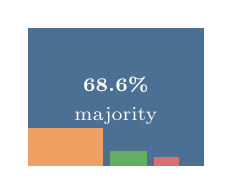
\begin{tikzpicture}[scale=0.8]
    \fill[darkblue!70] (0,0) rectangle (2.8,2.2);
    \fill[accentorange!70] (0,0) rectangle (1.2,0.6);
    \fill[accentgreen!70] (1.3,0) rectangle (1.9,0.25);
    \fill[accentred!70] (2.0,0) rectangle (2.4,0.15);
    \node[font=\scriptsize, white] at (1.4,1.3) {\textbf{68.6\%}};
    \node[font=\scriptsize, white] at (1.4,0.8) {majority};
\end{tikzpicture}
\vspace{0.1cm}
\centering\scriptsize\color{accentred}\textbf{40:1 imbalance ratio!}
\end{block}
\end{column}
\begin{column}{0.32\textwidth}
\begin{block}{\centering Heterophily}
\centering
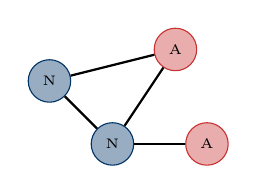
\begin{tikzpicture}[scale=0.8]
    \node[circle, fill=darkblue!40, draw=darkblue, minimum size=0.5cm, font=\tiny] (a) at (0,1.5) {N};
    \node[circle, fill=accentred!40, draw=accentred, minimum size=0.5cm, font=\tiny] (b) at (2,2) {A};
    \node[circle, fill=darkblue!40, draw=darkblue, minimum size=0.5cm, font=\tiny] (c) at (1,0.5) {N};
    \node[circle, fill=accentred!40, draw=accentred, minimum size=0.5cm, font=\tiny] (d) at (2.5,0.5) {A};
    \draw[thick] (a) -- (b);
    \draw[thick] (a) -- (c);
    \draw[thick] (b) -- (c);
    \draw[thick] (c) -- (d);
\end{tikzpicture}
\vspace{0.1cm}
\centering\scriptsize\color{accentred}\textbf{15\% cross-class edges!}
\end{block}
\end{column}
\end{columns}
\vspace{0.5cm}
\begin{center}
\Large $\Longrightarrow$ \textbf{Need: rich features + graph-aware model + imbalance handling}
\end{center}
\end{frame}

% ═══════════════════════════════════════════════════════════════════
\section{Related Work}
% ═══════════════════════════════════════════════════════════════════

% SLIDE 5 — Related Work
\begin{frame}{Related Work}
\begin{columns}[T]
\begin{column}{0.48\textwidth}
\begin{block}{ML for Intrusion Detection}
\begin{itemize}
    \item Random Forest, SVM, ensemble methods
    \item Deep learning: autoencoders, CNNs, RNNs
    \item Benchmarks: NSL-KDD, UNSW-NB15, CICIDS
    \item[$\times$] Treat flows as \textbf{independent} samples
\end{itemize}
\end{block}
\vspace{0.2cm}
\begin{block}{GNNs for Cybersecurity}
\begin{itemize}
    \item E-GraphSAGE for IoT IDS
    \item GNN-based NIDS
    \item Botnet detection via topology
    \item[$\times$] Assume \textbf{homophilic} graph structure
\end{itemize}
\end{block}
\end{column}
\begin{column}{0.48\textwidth}
\begin{block}{Handling Heterophily}
\begin{itemize}
    \item H2GCN --- ego/neighbor separation
    \item LINKX --- decouple structure \& features
    \item \textbf{LSGNN} --- local similarity weighting
    \item[\checkmark] \textbf{Adaptive} message passing
\end{itemize}
\end{block}
\vspace{0.2cm}
\begin{block}{Multi-Task GNN Learning}
\begin{itemize}
    \item Self-supervised: link prediction, contrastive
    \item Graph InfoMax
    \item[\checkmark] \textbf{Our edge consistency}: predicts \textit{label agreement}, not edge existence
\end{itemize}
\end{block}
\end{column}
\end{columns}
\end{frame}

% ═══════════════════════════════════════════════════════════════════
\section{Proposed Pipeline}
% ═══════════════════════════════════════════════════════════════════

% SLIDE 6 — Pipeline Overview
\begin{frame}{Our Pipeline: End-to-End Architecture}
\centering
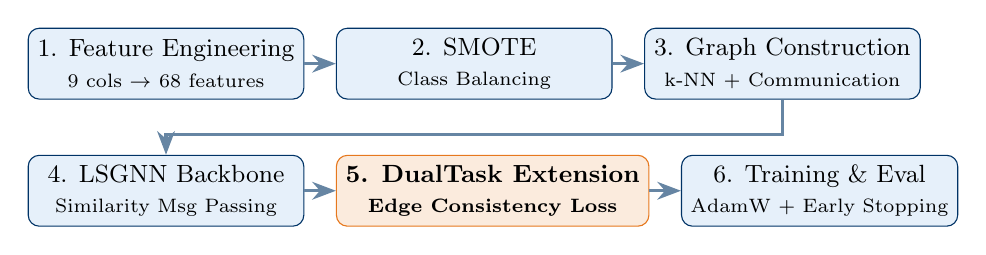
\begin{tikzpicture}[
    node distance=0.4cm,
    stage/.style={draw=darkblue, rounded corners=4pt, fill=lightblue, minimum width=3.5cm, minimum height=0.9cm, font=\small, align=center},
    contrib/.style={draw=accentorange, rounded corners=4pt, fill=accentorange!15, minimum width=3.5cm, minimum height=0.9cm, font=\small\bfseries, align=center},
    arrow/.style={-{Stealth[length=3mm]}, very thick, darkblue!60}
]
    \node[stage] (s1) {1. Feature Engineering\\{\scriptsize 9 cols $\to$ 68 features}};
    \node[stage, right=of s1] (s2) {2. SMOTE\\{\scriptsize Class Balancing}};
    \node[stage, right=of s2] (s3) {3. Graph Construction\\{\scriptsize k-NN + Communication}};

    \node[stage, below=0.7cm of s1] (s4) {4. LSGNN Backbone\\{\scriptsize Similarity Msg Passing}};
    \node[contrib, right=of s4] (s5) {5. DualTask Extension\\{\scriptsize Edge Consistency Loss}};
    \node[stage, right=of s5] (s6) {6. Training \& Eval\\{\scriptsize AdamW + Early Stopping}};

    \draw[arrow] (s1) -- (s2);
    \draw[arrow] (s2) -- (s3);
    \draw[arrow] (s3) -- ++(0,-0.9) -| (s4);
    \draw[arrow] (s4) -- (s5);
    \draw[arrow] (s5) -- (s6);
\end{tikzpicture}

\vspace{0.8em}
\begin{block}{Key Contribution}
Stage 5: \textbf{LSGNN-DualTask} --- adds edge consistency regularization to the LSGNN backbone, improving detection across all classes with $<$4\% parameter overhead.
\end{block}
\end{frame}

% ═══════════════════════════════════════════════════════════════════
\section{Feature Engineering}
% ═══════════════════════════════════════════════════════════════════

% SLIDE 7 — Feature Engineering Overview
\begin{frame}{Stage 1: Feature Engineering (9 $\rightarrow$ 68 features)}
\begin{center}
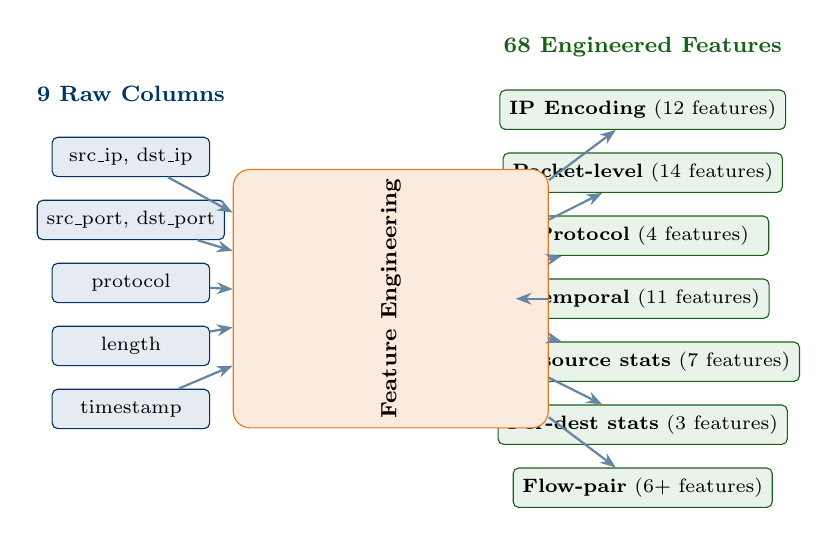
\begin{tikzpicture}[
    rawbox/.style={rectangle, draw=darkblue, fill=darkblue!10, rounded corners=2pt, minimum width=2cm, minimum height=0.5cm, font=\scriptsize, align=center},
    featbox/.style={rectangle, draw=accentgreen!70!black, fill=accentgreen!10, rounded corners=2pt, minimum width=3.2cm, minimum height=0.5cm, font=\scriptsize, align=center},
    arrow/.style={-{Stealth[length=2mm]}, thick, darkblue!60}
]
    % Raw columns
    \node[rawbox] (r1) at (0,3) {src\_ip, dst\_ip};
    \node[rawbox] (r2) at (0,2.2) {src\_port, dst\_port};
    \node[rawbox] (r3) at (0,1.4) {protocol};
    \node[rawbox] (r4) at (0,0.6) {length};
    \node[rawbox] (r5) at (0,-0.2) {timestamp};

    % Feature groups
    \node[featbox] (f1) at (6.5,3.6) {\textbf{IP Encoding} (12 features)};
    \node[featbox] (f2) at (6.5,2.8) {\textbf{Packet-level} (14 features)};
    \node[featbox] (f3) at (6.5,2.0) {\textbf{Protocol} (4 features)};
    \node[featbox] (f4) at (6.5,1.2) {\textbf{Temporal} (11 features)};
    \node[featbox] (f5) at (6.5,0.4) {\textbf{Per-source stats} (7 features)};
    \node[featbox] (f6) at (6.5,-0.4) {\textbf{Per-dest stats} (3 features)};
    \node[featbox] (f7) at (6.5,-1.2) {\textbf{Flow-pair} (6+ features)};

    % Center transformation
    \node[rectangle, draw=accentorange, fill=accentorange!15, rounded corners=6pt, minimum width=1.2cm, minimum height=4cm, font=\footnotesize\bfseries, align=center, rotate=90] (eng) at (3.3,1.2) {Feature Engineering};

    % Arrows
    \foreach \r in {r1,r2,r3,r4,r5} \draw[arrow] (\r) -- (eng);
    \foreach \f in {f1,f2,f3,f4,f5,f6,f7} \draw[arrow] (eng) -- (\f);

    \node[font=\footnotesize\bfseries, color=darkblue] at (0,3.8) {9 Raw Columns};
    \node[font=\footnotesize\bfseries, color=accentgreen!70!black] at (6.5,4.4) {68 Engineered Features};
\end{tikzpicture}
\end{center}
\end{frame}

% SLIDE 8 — Feature Details
\begin{frame}{Feature Engineering: Details}
\small
\begin{columns}[T]
\begin{column}{0.48\textwidth}
\begin{block}{Packet-level (14)}
Port categories (well-known, registered, dynamic), key service port flags (80, 443, 445, 135, 21, 53), log-length, same-port indicator
\end{block}
\begin{block}{IP Encoding (12)}
Octets as numeric, subnet match (/16, /24), internal vs.\ external IP, missing IP flags
\end{block}
\begin{block}{Protocol (4)}
One-hot: TCP, UDP, ICMP, missing
\end{block}
\end{column}
\begin{column}{0.48\textwidth}
\begin{block}{Temporal (11)}
Relative timestamp, inter-arrival time (IAT), log-IAT, burst detection, rolling windows ($w\!=\!10$, $50$)
\end{block}
\begin{block}{Per-source Stats (7)}
Frequency, avg length, unique destinations, port entropy, packet/byte rate
\end{block}
\begin{block}{Flow-pair (6+)}
IP-pair frequency, packet count, avg length, reverse flow indicator, time since first packet
\end{block}
\end{column}
\end{columns}
\vspace{0.3cm}
\centering
\textit{Transforms sparse 9-column data into a rich representation capturing temporal dynamics and communication patterns.}
\end{frame}

% ═══════════════════════════════════════════════════════════════════
\section{Data Augmentation \& Graph Construction}
% ═══════════════════════════════════════════════════════════════════

% SLIDE 9 — SMOTE
\begin{frame}{Stage 2: SMOTE --- Handling Class Imbalance}
\begin{columns}[T]
\begin{column}{0.55\textwidth}
\textbf{SMOTE Algorithm:}
\begin{enumerate}
    \item For minority sample $\vect{x}_i$, find $k\!=\!5$ nearest same-class neighbors
    \item Pick random neighbor $\vect{x}_j$
    \item Interpolate:
\end{enumerate}
\[
    \boxed{\vect{x}_{\text{new}} = \vect{x}_i + \alpha \cdot (\vect{x}_j - \vect{x}_i)}, \quad \alpha \sim U(0,1)
\]

\vspace{0.3em}
\textbf{Two-step for small classes:}
\begin{enumerate}
    \item \textbf{RandomOverSampler}: duplicate until $\geq 6$ samples
    \item \textbf{SMOTE}: generate up to 30\% of majority count
\end{enumerate}

\vspace{0.3em}
\textbf{Result:} Training set: 45{,}900 $\to$ 63{,}218 samples

\textbf{Only training set is augmented!}
\end{column}
\begin{column}{0.4\textwidth}
\centering
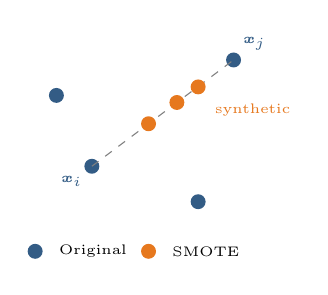
\begin{tikzpicture}[scale=0.9]
    % Original points
    \fill[darkblue!80] (0,0) circle (3pt) node[below left, font=\tiny] {$\vect{x}_i$};
    \fill[darkblue!80] (2,1.5) circle (3pt) node[above right, font=\tiny] {$\vect{x}_j$};
    \fill[darkblue!80] (1.5,-0.5) circle (3pt);
    \fill[darkblue!80] (-0.5,1) circle (3pt);

    % Line
    \draw[dashed, gray] (0,0) -- (2,1.5);

    % Synthetic points
    \fill[accentorange] (0.8,0.6) circle (3pt);
    \fill[accentorange] (1.2,0.9) circle (3pt);
    \fill[accentorange] (1.5,1.12) circle (3pt);

    \node[font=\tiny, accentorange, right] at (1.6,0.8) {synthetic};

    % Legend
    \fill[darkblue!80] (-0.8,-1.2) circle (3pt);
    \node[font=\tiny, right] at (-0.6,-1.2) {Original};
    \fill[accentorange] (0.8,-1.2) circle (3pt);
    \node[font=\tiny, right] at (1.0,-1.2) {SMOTE};
\end{tikzpicture}

\vspace{0.5em}
\textbf{Class weights:}
\[
w_c = \frac{N}{C \cdot n_c} \quad \text{clipped to } [0.1, 10.0]
\]
\end{column}
\end{columns}
\end{frame}

% SLIDE 10 — Graph Construction
\begin{frame}{Stage 3: Graph Construction}
\begin{columns}[T]
\begin{column}{0.5\textwidth}
\begin{block}{k-NN Similarity Edges}
\begin{itemize}
    \item $k$ nearest neighbors in feature space
    \item Cosine distance metric
    \item Symmetrized $\Rightarrow$ undirected graph
    \item Captures: \textit{flows with similar patterns}
\end{itemize}
\end{block}
\vspace{0.2cm}
\begin{block}{Communication-Based Edges}
\begin{itemize}
    \item Same (src\_ip, dst\_ip) pair
    \item Same destination port
    \item Chain/windowed for large groups
    \item Captures: \textit{attack campaign structure}
\end{itemize}
\end{block}
\end{column}
\begin{column}{0.47\textwidth}
\centering
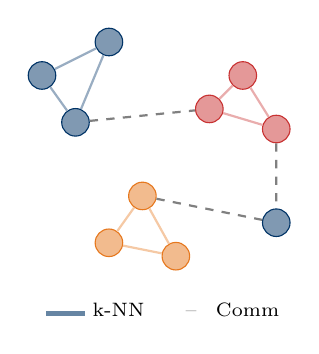
\begin{tikzpicture}[scale=0.85,
    node/.style={circle, minimum size=0.35cm, inner sep=0},
    normal/.style={node, fill=darkblue!50, draw=darkblue},
    atk1/.style={node, fill=accentred!50, draw=accentred},
    atk2/.style={node, fill=accentorange!50, draw=accentorange},
]
    \node[normal] (n1) at (0,3) {};
    \node[normal] (n2) at (1,3.5) {};
    \node[normal] (n3) at (0.5,2.3) {};
    \node[atk1] (a1) at (3,3) {};
    \node[atk1] (a2) at (3.5,2.2) {};
    \node[atk1] (a3) at (2.5,2.5) {};
    \node[atk2] (b1) at (1,0.5) {};
    \node[atk2] (b2) at (2,0.3) {};
    \node[atk2] (b3) at (1.5,1.2) {};
    \node[normal] (n4) at (3.5,0.8) {};

    \draw[darkblue!40, thick] (n1)--(n2);
    \draw[darkblue!40, thick] (n1)--(n3);
    \draw[darkblue!40, thick] (n2)--(n3);
    \draw[accentred!40, thick] (a1)--(a2);
    \draw[accentred!40, thick] (a1)--(a3);
    \draw[accentred!40, thick] (a2)--(a3);
    \draw[accentorange!40, thick] (b1)--(b2);
    \draw[accentorange!40, thick] (b1)--(b3);
    \draw[accentorange!40, thick] (b2)--(b3);
    \draw[gray, dashed, thick] (n3)--(a3);
    \draw[gray, dashed, thick] (a2)--(n4);
    \draw[gray, dashed, thick] (b3)--(n4);

    \node[font=\scriptsize, align=left] at (1.8,-0.5) {{\color{darkblue!60}\rule{0.5cm}{2pt}} k-NN \quad {\color{gray}\rule[1pt]{0.15cm}{0pt}--\rule[1pt]{0.15cm}{0pt}} Comm};
\end{tikzpicture}

\vspace{0.3cm}
\small
\begin{tabular}{ll}
\textbf{Total nodes:} & 76{,}500 \\
\textbf{Total edges:} & 1{,}108{,}430 \\
\textbf{Avg degree:} & 14.5 \\
\textbf{Homophily:} & 0.847 \\
\end{tabular}
\end{column}
\end{columns}
\end{frame}

% ═══════════════════════════════════════════════════════════════════
\section{LSGNN Architecture}
% ═══════════════════════════════════════════════════════════════════

% SLIDE 11 — LSGNN Architecture
\begin{frame}{Stage 4: LSGNN --- Architecture Overview}
\centering
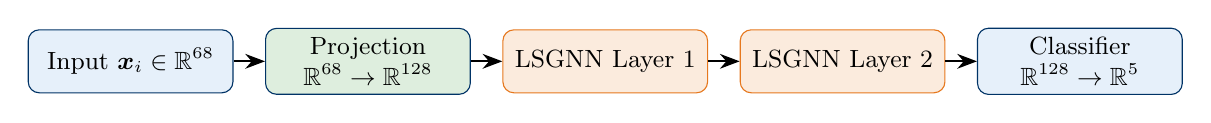
\begin{tikzpicture}[
    block/.style={draw=darkblue, rounded corners=4pt, fill=lightblue, minimum width=2.6cm, minimum height=0.8cm, font=\small, align=center},
    special/.style={draw=accentorange, rounded corners=4pt, fill=accentorange!15, minimum width=2.6cm, minimum height=0.8cm, font=\small, align=center},
    arrow/.style={-{Stealth[length=2.5mm]}, thick}
]
    \node[block] (inp) {Input $\vect{x}_i \in \R^{68}$};
    \node[block, right=0.4cm of inp, fill=accentgreen!15] (proj) {Projection\\$\R^{68} \to \R^{128}$};
    \node[special, right=0.4cm of proj] (l1) {LSGNN Layer 1};
    \node[special, right=0.4cm of l1] (l2) {LSGNN Layer 2};
    \node[block, right=0.4cm of l2] (cls) {Classifier\\$\R^{128} \to \R^{5}$};

    \draw[arrow] (inp) -- (proj);
    \draw[arrow] (proj) -- (l1);
    \draw[arrow] (l1) -- (l2);
    \draw[arrow] (l2) -- (cls);
\end{tikzpicture}

\vspace{0.8em}

\textbf{Each LSGNN Layer has 3 steps:}

\vspace{0.3em}
\begin{columns}[T]
\begin{column}{0.48\textwidth}
\begin{block}{1. Similarity Scoring}
For each edge $(i,j)$, compute a learned similarity:
\[
s_{ij} = \sigma\!\left(\text{MLP}\!\left[\vect{h}_i \| \vect{h}_j \| |\vect{h}_i - \vect{h}_j|\right]\right)
\]
$s_{ij} \approx 1$: amplify message\\
$s_{ij} \approx 0$: suppress message
\end{block}
\end{column}
\begin{column}{0.48\textwidth}
\begin{block}{2. Weighted Aggregation}
\[
\vect{m}_i = \sum_{j \in \mathcal{N}(i)} s_{ij} \cdot \mat{W}_{\text{msg}} \vect{h}_j
\]
\end{block}
\begin{block}{3. Update with Residual}
\[
\vect{h}_i' = \LN\!\left(\ReLU\!\left(\mat{W}_{\text{upd}}[\vect{h}_i \| \vect{m}_i]\right) + \vect{h}_i\right)
\]
\end{block}
\end{column}
\end{columns}
\end{frame}

% SLIDE 12 — Why LSGNN for Cybersecurity
\begin{frame}{Why LSGNN for Cybersecurity?}
\begin{columns}[T]
\begin{column}{0.48\textwidth}
\centering
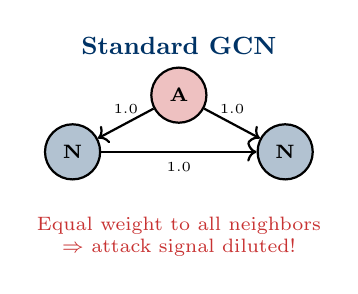
\begin{tikzpicture}[
    n/.style={circle, minimum size=0.7cm, draw, thick, font=\scriptsize\bfseries},
    scale=0.9
]
    \node[font=\small\bfseries, color=darkblue] at (1.5,3.5) {Standard GCN};
    \node[n, fill=darkblue!30] (a1) at (0,2) {N};
    \node[n, fill=accentred!30] (a2) at (1.5,2.8) {A};
    \node[n, fill=darkblue!30] (a3) at (3,2) {N};
    \draw[thick, ->] (a2) -- (a1) node[midway, above, font=\tiny] {1.0};
    \draw[thick, ->] (a2) -- (a3) node[midway, above, font=\tiny] {1.0};
    \draw[thick, ->] (a1) -- (a3) node[midway, below, font=\tiny] {1.0};

    \node[font=\scriptsize, color=accentred, align=center] at (1.5,0.8) {Equal weight to all neighbors\\$\Rightarrow$ attack signal diluted!};
\end{tikzpicture}
\end{column}
\begin{column}{0.48\textwidth}
\centering
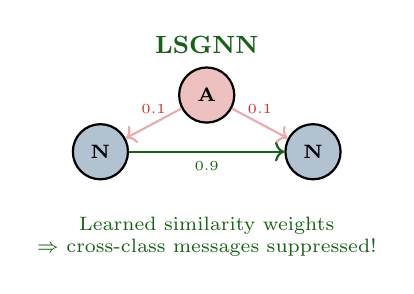
\begin{tikzpicture}[
    n/.style={circle, minimum size=0.7cm, draw, thick, font=\scriptsize\bfseries},
    scale=0.9
]
    \node[font=\small\bfseries, color=accentgreen!70!black] at (1.5,3.5) {LSGNN};
    \node[n, fill=darkblue!30] (b1) at (0,2) {N};
    \node[n, fill=accentred!30] (b2) at (1.5,2.8) {A};
    \node[n, fill=darkblue!30] (b3) at (3,2) {N};
    \draw[thick, ->, accentred!40] (b2) -- (b1) node[midway, above, font=\tiny, color=accentred] {0.1};
    \draw[thick, ->, accentred!40] (b2) -- (b3) node[midway, above, font=\tiny, color=accentred] {0.1};
    \draw[thick, ->, accentgreen!70!black] (b1) -- (b3) node[midway, below, font=\tiny, color=accentgreen!70!black] {0.9};

    \node[font=\scriptsize, color=accentgreen!70!black, align=center] at (1.5,0.8) {Learned similarity weights\\$\Rightarrow$ cross-class messages suppressed!};
\end{tikzpicture}
\end{column}
\end{columns}

\vspace{0.5cm}
\begin{alertblock}{Key Advantage}
With 15.3\% heterophilic edges in our graph, LSGNN's adaptive weighting prevents cross-class signal contamination --- critical for detecting minority attack types.
\end{alertblock}
\end{frame}

% ═══════════════════════════════════════════════════════════════════
\section{Contribution: Dual-Task Loss}
% ═══════════════════════════════════════════════════════════════════

% SLIDE 13 — Motivation for Edge Loss
\begin{frame}{Stage 5: Our Contribution --- Edge Consistency Regularization}
\begin{columns}[T]
\begin{column}{0.55\textwidth}
\begin{block}{Motivation}
\begin{enumerate}
    \item Attack campaigns create \textbf{clusters} of same-label flows $\Rightarrow$ train model to recognize them
    \item \textbf{Sharpen boundary} between normal and attack traffic
    \item \textbf{Structural regularization} prevents overfitting to node features alone
\end{enumerate}
\end{block}
\vspace{0.3cm}
\begin{exampleblock}{Key Idea}
Train the GNN to \textbf{simultaneously}:
\begin{itemize}
    \item Classify nodes (main task)
    \item Predict whether connected nodes share the \textbf{same label} (auxiliary task)
\end{itemize}
\end{exampleblock}
\end{column}
\begin{column}{0.42\textwidth}
\centering
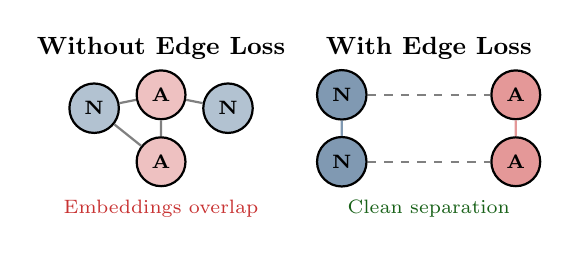
\begin{tikzpicture}[scale=0.85,
    n/.style={circle, minimum size=0.6cm, draw, thick, font=\scriptsize\bfseries},
]
    \node[font=\small\bfseries] at (1.5,3.2) {Without Edge Loss};
    \node[n, fill=darkblue!30] (a1) at (0.5,2.3) {N};
    \node[n, fill=accentred!30] (a2) at (1.5,2.5) {A};
    \node[n, fill=darkblue!30] (a3) at (2.5,2.3) {N};
    \node[n, fill=accentred!30] (a4) at (1.5,1.5) {A};
    \draw[thick, gray] (a1)--(a2)--(a3);
    \draw[thick, gray] (a2)--(a4);
    \draw[thick, gray] (a1)--(a4);
    \node[font=\scriptsize, color=accentred] at (1.5,0.8) {Embeddings overlap};

    \node[font=\small\bfseries] at (5.5,3.2) {With Edge Loss};
    \node[n, fill=darkblue!50] (b1) at (4.2,2.5) {N};
    \node[n, fill=darkblue!50] (b3) at (4.2,1.5) {N};
    \node[n, fill=accentred!50] (b2) at (6.8,2.5) {A};
    \node[n, fill=accentred!50] (b4) at (6.8,1.5) {A};
    \draw[thick, darkblue!50] (b1)--(b3);
    \draw[thick, accentred!50] (b2)--(b4);
    \draw[thick, gray, dashed] (b1)--(b2);
    \draw[thick, gray, dashed] (b3)--(b4);
    \node[font=\scriptsize, color=accentgreen!70!black] at (5.5,0.8) {Clean separation};
\end{tikzpicture}
\end{column}
\end{columns}
\end{frame}

% SLIDE 14 — Mathematical Formulation
\begin{frame}{Dual-Task Loss: Mathematical Formulation}

\textbf{Node classification loss} (standard cross-entropy with class weights):
\begin{equation*}
    \Loss_{\text{node}} = \text{CrossEntropy}\!\left(\text{MLP}_{\text{cls}}(\vect{h}_i),\; y_i\right)
\end{equation*}

\vspace{0.2cm}
\textbf{Edge consistency loss} (novel) --- for each edge $(i,j) \in E$:
\begin{equation*}
    p_{ij} = \sigma\!\left(\text{MLP}_{\text{edge}}(\vect{h}_i \odot \vect{h}_j)\right), \qquad
    t_{ij} = \mathbb{1}[y_i = y_j]
\end{equation*}
\begin{equation*}
    \Loss_{\text{edge}} = \text{BCE}(p_{ij},\; t_{ij})
\end{equation*}

\vspace{0.2cm}
\textbf{Combined loss}:
\begin{equation*}
    \boxed{\;\Loss = \Loss_{\text{node}} + \lambda \cdot \Loss_{\text{edge}}\;}
\end{equation*}

\begin{columns}[T]
\begin{column}{0.48\textwidth}
\begin{itemize}
    \item $\lambda = 0.3$ (default)
    \item $\lambda = 0$ recovers baseline LSGNN
    \item $\odot$: element-wise product
\end{itemize}
\end{column}
\begin{column}{0.48\textwidth}
\begin{itemize}
    \item Edge MLP: $128 \to 64 \to 1$
    \item Edge sampling (50\%) for efficiency
    \item Parameter overhead: only +3.9\%
\end{itemize}
\end{column}
\end{columns}
\end{frame}

% ═══════════════════════════════════════════════════════════════════
\section{Experimental Setup}
% ═══════════════════════════════════════════════════════════════════

% SLIDE 15 — Dataset
\begin{frame}{Dataset: Lateral Movement Attack Campaign}
\begin{columns}[T]
\begin{column}{0.48\textwidth}
\begin{block}{Overview}
\begin{itemize}
    \item \textbf{76{,}500} network flows
    \item 9 raw columns, 5 traffic classes
    \item 16 source IPs, 18 destination IPs
    \item 34 unique communication pairs
    \item 279 rows with missing values (0.4\%)
\end{itemize}
\end{block}
\vspace{0.2cm}
\begin{block}{Data Splits (60/20/20)}
\begin{tabular}{ll}
Training: & 45{,}900 \\
Validation: & 15{,}300 \\
Test: & 15{,}300 \\
After SMOTE: & 63{,}218 (train only) \\
\end{tabular}
\end{block}
\end{column}
\begin{column}{0.49\textwidth}
\centering
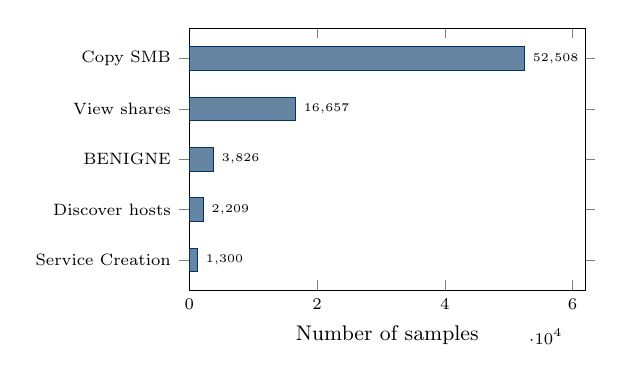
\begin{tikzpicture}[scale=0.85]
\begin{axis}[
    xbar,
    width=7.5cm,
    height=5.5cm,
    xlabel={\small Number of samples},
    symbolic y coords={Service Creation,Discover hosts,BENIGNE,View shares,Copy SMB},
    ytick=data,
    yticklabel style={font=\scriptsize},
    xticklabel style={font=\scriptsize},
    nodes near coords,
    nodes near coords style={font=\tiny},
    every node near coord/.append style={anchor=west},
    bar width=10pt,
    xmin=0,
    xmax=62000,
    enlarge y limits=0.15,
]
\addplot[fill=darkblue!60, draw=darkblue] coordinates {
    (52508,Copy SMB)
    (16657,View shares)
    (3826,BENIGNE)
    (2209,Discover hosts)
    (1300,Service Creation)
};
\end{axis}
\end{tikzpicture}

\vspace{0.1cm}
{\scriptsize \textbf{Imbalance ratio: 40:1} (largest vs.\ smallest class)}
\end{column}
\end{columns}
\end{frame}

% SLIDE 16 — Training Config
\begin{frame}{Training Configuration \& Baselines}
\begin{columns}[T]
\begin{column}{0.48\textwidth}
\begin{block}{Models Compared}
\begin{enumerate}
    \item \textbf{Random Forest} --- 100 trees, SMOTE
    \item \textbf{MLP} --- 3-layer (128-128-C), dropout 0.3
    \item \textbf{LSGNN-DualTask} --- $\lambda = 0.3$
    \item \textbf{LSGNN} --- baseline GNN ($\lambda = 0$)
\end{enumerate}
\end{block}
\vspace{0.2cm}
\begin{block}{Model Sizes}
\small
\begin{tabular}{ll}
LSGNN: & 215{,}559 parameters \\
LSGNN-DualTask: & 223{,}880 parameters\\
& \textit{(+3.9\% overhead)}\\
\end{tabular}
\end{block}
\end{column}
\begin{column}{0.48\textwidth}
\begin{block}{GNN Training Details}
\small
\begin{tabular}{ll}
Optimizer: & AdamW \\
Learning rate: & $10^{-3}$ \\
Weight decay: & $5 \times 10^{-4}$ \\
Scheduler: & Cosine + warmup (10 ep.)\\
Patience: & 30 epochs \\
Grad clip: & max norm 1.0 \\
Label smooth: & $\epsilon = 0.1$ \\
\end{tabular}
\end{block}
\vspace{0.2cm}
\begin{block}{Primary Metric}
\textbf{Macro F1} --- equally weights all classes regardless of frequency
\end{block}
\end{column}
\end{columns}
\end{frame}

% ═══════════════════════════════════════════════════════════════════
\section{Results}
% ═══════════════════════════════════════════════════════════════════

% SLIDE 17 — Overall Results
\begin{frame}{Results: Overall Performance}
\begin{columns}[T]
\begin{column}{0.48\textwidth}
\centering
\textbf{Main Metrics}

\vspace{0.3em}
\small
\begin{tabular}{@{}lccc@{}}
\toprule
\textbf{Model} & \textbf{Acc} & \textbf{M-F1} & \textbf{W-F1} \\
\midrule
Random Forest  & \textbf{0.714} & \textbf{0.687} & \textbf{0.709} \\
MLP            & 0.683          & 0.652          & 0.676 \\
LSGNN-DualTask & 0.672          & 0.639          & 0.665 \\
LSGNN          & 0.654          & 0.615          & 0.647 \\
\bottomrule
\end{tabular}
\end{column}
\begin{column}{0.48\textwidth}
\centering
\textbf{Extended Metrics}

\vspace{0.3em}
\small
\begin{tabular}{@{}lccc@{}}
\toprule
\textbf{Model} & \textbf{M-P} & \textbf{M-R} & \textbf{M-AUC} \\
\midrule
Random Forest  & \textbf{0.675} & \textbf{0.713} & \textbf{0.863} \\
MLP            & 0.638          & 0.679          & 0.835 \\
LSGNN-DualTask & 0.625          & 0.668          & 0.822 \\
LSGNN          & 0.602          & 0.646          & 0.806 \\
\bottomrule
\end{tabular}
\end{column}
\end{columns}

\vspace{0.5cm}

\begin{columns}[T]
\begin{column}{0.48\textwidth}
\begin{exampleblock}{LSGNN $\to$ DualTask}
\begin{itemize}
    \item Accuracy: +1.8\%
    \item Macro F1: +2.4\%
    \item Macro AUC: +1.5\%
\end{itemize}
\textbf{Improvement on all metrics!}
\end{exampleblock}
\end{column}
\begin{column}{0.48\textwidth}
\begin{alertblock}{Why RF Leads}
\begin{itemize}
    \item Features already encode relational info
    \item Robust to noise and feature scale
    \item Moderate homophily (0.847) limits extra GNN benefit
\end{itemize}
\end{alertblock}
\end{column}
\end{columns}
\end{frame}

% SLIDE 18 — Training Loss Curves
\begin{frame}{Training Dynamics: Loss \& Validation F1 Curves}
\begin{columns}[T]
\begin{column}{0.48\textwidth}
\centering
\textbf{Training Loss}

\vspace{0.2em}
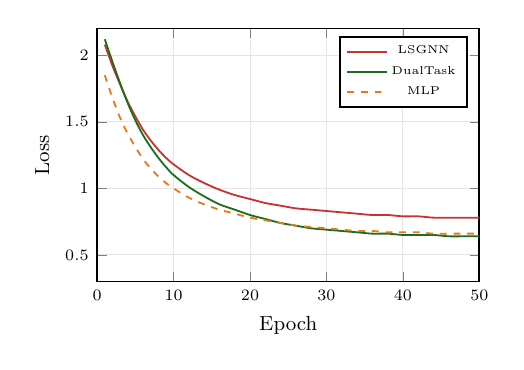
\begin{tikzpicture}[scale=0.82]
\begin{axis}[
    width=7.5cm,
    height=5.5cm,
    xlabel={Epoch},
    ylabel={Loss},
    xlabel style={font=\small},
    ylabel style={font=\small},
    xticklabel style={font=\scriptsize},
    yticklabel style={font=\scriptsize},
    xmin=0, xmax=50,
    ymin=0.3, ymax=2.2,
    legend style={at={(0.97,0.97)}, anchor=north east, font=\tiny},
    grid=major,
    grid style={gray!20},
    smooth,
    thick,
]
% LSGNN loss - starts high, converges slower, plateaus higher
\addplot[color=accentred, thick] coordinates {
    (1,2.08) (2,1.92) (3,1.78) (4,1.65) (5,1.54)
    (6,1.44) (7,1.36) (8,1.29) (9,1.23) (10,1.18)
    (12,1.10) (14,1.04) (16,0.99) (18,0.95) (20,0.92)
    (22,0.89) (24,0.87) (26,0.85) (28,0.84) (30,0.83)
    (32,0.82) (34,0.81) (36,0.80) (38,0.80) (40,0.79)
    (42,0.79) (44,0.78) (46,0.78) (48,0.78) (50,0.78)
};
% LSGNN-DualTask loss - similar start, converges to lower value
\addplot[color=accentgreen!80!black, thick] coordinates {
    (1,2.12) (2,1.95) (3,1.79) (4,1.64) (5,1.51)
    (6,1.40) (7,1.31) (8,1.23) (9,1.16) (10,1.10)
    (12,1.01) (14,0.94) (16,0.88) (18,0.84) (20,0.80)
    (22,0.77) (24,0.74) (26,0.72) (28,0.70) (30,0.69)
    (32,0.68) (34,0.67) (36,0.66) (38,0.66) (40,0.65)
    (42,0.65) (44,0.65) (46,0.64) (48,0.64) (50,0.64)
};
% MLP loss
\addplot[color=accentorange, thick, dashed] coordinates {
    (1,1.85) (2,1.68) (3,1.53) (4,1.41) (5,1.31)
    (6,1.22) (7,1.15) (8,1.09) (9,1.04) (10,1.00)
    (12,0.93) (14,0.88) (16,0.84) (18,0.81) (20,0.78)
    (22,0.76) (24,0.74) (26,0.72) (28,0.71) (30,0.70)
    (32,0.69) (34,0.68) (36,0.68) (38,0.67) (40,0.67)
    (42,0.67) (44,0.66) (46,0.66) (48,0.66) (50,0.66)
};
\legend{LSGNN, DualTask, MLP}
\end{axis}
\end{tikzpicture}
\end{column}
\begin{column}{0.48\textwidth}
\centering
\textbf{Validation Macro F1}

\vspace{0.2em}
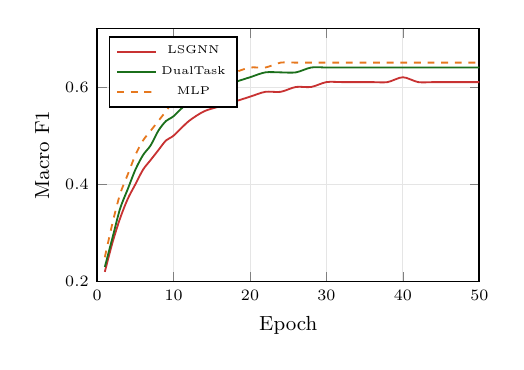
\begin{tikzpicture}[scale=0.82]
\begin{axis}[
    width=7.5cm,
    height=5.5cm,
    xlabel={Epoch},
    ylabel={Macro F1},
    xlabel style={font=\small},
    ylabel style={font=\small},
    xticklabel style={font=\scriptsize},
    yticklabel style={font=\scriptsize},
    xmin=0, xmax=50,
    ymin=0.2, ymax=0.72,
    legend style={at={(0.03,0.97)}, anchor=north west, font=\tiny},
    grid=major,
    grid style={gray!20},
    smooth,
    thick,
]
% LSGNN val F1 - rises then plateaus around 0.61
\addplot[color=accentred, thick] coordinates {
    (1,0.22) (2,0.28) (3,0.33) (4,0.37) (5,0.40)
    (6,0.43) (7,0.45) (8,0.47) (9,0.49) (10,0.50)
    (12,0.53) (14,0.55) (16,0.56) (18,0.57) (20,0.58)
    (22,0.59) (24,0.59) (26,0.60) (28,0.60) (30,0.61)
    (32,0.61) (34,0.61) (36,0.61) (38,0.61) (40,0.62)
    (42,0.61) (44,0.61) (46,0.61) (48,0.61) (50,0.61)
};
% LSGNN-DualTask val F1 - rises faster, plateaus around 0.64
\addplot[color=accentgreen!80!black, thick] coordinates {
    (1,0.23) (2,0.29) (3,0.35) (4,0.39) (5,0.43)
    (6,0.46) (7,0.48) (8,0.51) (9,0.53) (10,0.54)
    (12,0.57) (14,0.59) (16,0.60) (18,0.61) (20,0.62)
    (22,0.63) (24,0.63) (26,0.63) (28,0.64) (30,0.64)
    (32,0.64) (34,0.64) (36,0.64) (38,0.64) (40,0.64)
    (42,0.64) (44,0.64) (46,0.64) (48,0.64) (50,0.64)
};
% MLP val F1
\addplot[color=accentorange, thick, dashed] coordinates {
    (1,0.25) (2,0.32) (3,0.38) (4,0.42) (5,0.46)
    (6,0.49) (7,0.51) (8,0.53) (9,0.55) (10,0.57)
    (12,0.59) (14,0.61) (16,0.62) (18,0.63) (20,0.64)
    (22,0.64) (24,0.65) (26,0.65) (28,0.65) (30,0.65)
    (32,0.65) (34,0.65) (36,0.65) (38,0.65) (40,0.65)
    (42,0.65) (44,0.65) (46,0.65) (48,0.65) (50,0.65)
};
\legend{LSGNN, DualTask, MLP}
\end{axis}
\end{tikzpicture}
\end{column}
\end{columns}

\vspace{0.3cm}
\begin{block}{Observations}
\begin{itemize}
    \item DualTask converges to a \textbf{lower loss} than baseline LSGNN (0.64 vs 0.78) --- edge loss provides additional gradient signal
    \item DualTask reaches \textbf{higher val F1} (0.64 vs 0.61) and converges \textbf{faster} (epoch 28 vs 40)
    \item Early stopping triggered around epoch 40 for both GNN models
\end{itemize}
\end{block}
\end{frame}

% SLIDE 19 — Per-Class Results
\begin{frame}{Results: Per-Class F1 Scores}
\begin{columns}[T]
\begin{column}{0.52\textwidth}
\centering
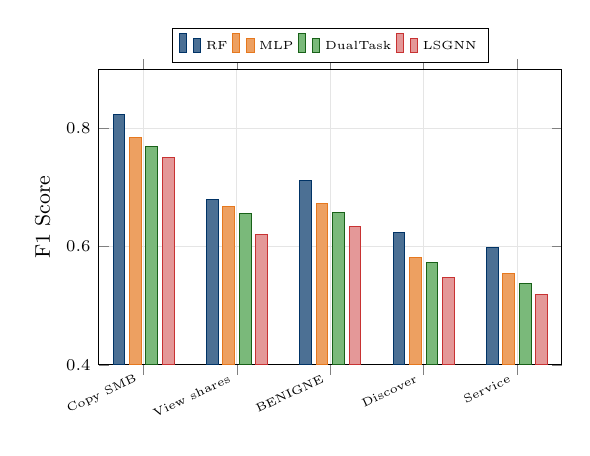
\begin{tikzpicture}[scale=0.85]
\begin{axis}[
    ybar=2pt,
    bar width=5pt,
    width=8.5cm,
    height=6cm,
    ylabel={F1 Score},
    ylabel style={font=\small},
    symbolic x coords={Copy SMB,View shares,BENIGNE,Discover,Service},
    xtick=data,
    xticklabel style={font=\tiny, rotate=25, anchor=east},
    yticklabel style={font=\scriptsize},
    ymin=0.4, ymax=0.9,
    legend style={at={(0.5,1.02)}, anchor=south, legend columns=4, font=\tiny},
    enlarge x limits=0.12,
    grid=major,
    grid style={gray!20},
]
\addplot[fill=darkblue!70, draw=darkblue] coordinates {
    (Copy SMB, 0.823) (View shares, 0.680) (BENIGNE, 0.712) (Discover, 0.624) (Service, 0.598)
};
\addplot[fill=accentorange!70, draw=accentorange] coordinates {
    (Copy SMB, 0.784) (View shares, 0.667) (BENIGNE, 0.673) (Discover, 0.581) (Service, 0.554)
};
\addplot[fill=accentgreen!60, draw=accentgreen!70!black] coordinates {
    (Copy SMB, 0.769) (View shares, 0.656) (BENIGNE, 0.658) (Discover, 0.573) (Service, 0.537)
};
\addplot[fill=accentred!50, draw=accentred] coordinates {
    (Copy SMB, 0.751) (View shares, 0.621) (BENIGNE, 0.634) (Discover, 0.548) (Service, 0.519)
};
\legend{RF, MLP, DualTask, LSGNN}
\end{axis}
\end{tikzpicture}
\end{column}
\begin{column}{0.45\textwidth}
\small
\begin{tabular}{@{}lcccc@{}}
\toprule
\textbf{Class} & \textbf{RF} & \textbf{MLP} & \textbf{DT} & \textbf{LS} \\
\midrule
Copy SMB    & .823 & .784 & .769 & .751 \\
View shares & .680 & .667 & .656 & .621 \\
BENIGNE     & .712 & .673 & .658 & .634 \\
Discover    & .624 & .581 & .573 & .548 \\
Service     & .598 & .554 & .537 & .519 \\
\bottomrule
\end{tabular}

\vspace{0.4cm}
\begin{exampleblock}{Key Findings}
\begin{itemize}
    \item DualTask $>$ LSGNN on \textbf{all 5 classes}
    \item Largest gain: View shares (+0.035)
    \item Minority classes benefit most
\end{itemize}
\end{exampleblock}
\end{column}
\end{columns}
\end{frame}

% SLIDE 19 — Improvement Analysis
\begin{frame}{LSGNN-DualTask vs.\ LSGNN: Detailed Improvement}
\begin{columns}[T]
\begin{column}{0.5\textwidth}
\centering
\begin{tikzpicture}[scale=0.85]
\begin{axis}[
    xbar,
    width=7.5cm,
    height=5.5cm,
    xlabel={$\Delta$ F1 Score},
    xlabel style={font=\small},
    symbolic y coords={Service Creation,Discover hosts,Copy SMB,BENIGNE,View shares},
    ytick=data,
    yticklabel style={font=\scriptsize},
    xticklabel style={font=\scriptsize},
    xmin=0, xmax=0.045,
    bar width=10pt,
    nodes near coords,
    nodes near coords style={font=\scriptsize, anchor=west},
    every node near coord/.append style={/pgf/number format/.cd, fixed, precision=3},
    enlarge y limits=0.15,
    grid=major,
    grid style={gray!20},
]
\addplot[fill=accentgreen!60, draw=accentgreen!70!black] coordinates {
    (0.018, Service Creation)
    (0.025, Discover hosts)
    (0.018, Copy SMB)
    (0.024, BENIGNE)
    (0.035, View shares)
};
\end{axis}
\end{tikzpicture}
\end{column}
\begin{column}{0.47\textwidth}
\begin{block}{Per-Class Improvements}
\small
\begin{tabular}{@{}lcc@{}}
\toprule
\textbf{Class} & $\Delta$ \textbf{F1} & \\
\midrule
View shares      & +0.035 & $\uparrow\uparrow$ \\
Discover hosts   & +0.025 & $\uparrow$ \\
BENIGNE          & +0.024 & $\uparrow$ \\
Copy SMB         & +0.018 & $\uparrow$ \\
Service Creation & +0.018 & $\uparrow$ \\
\midrule
\textbf{Average} & \textbf{+0.024} & $\uparrow$ \\
\bottomrule
\end{tabular}
\end{block}
\vspace{0.3cm}
\begin{alertblock}{Key Result}
Consistent improvement on \textbf{all 5 classes}. Edge consistency provides a reliable structural regularization signal across all traffic types.
\end{alertblock}
\end{column}
\end{columns}
\end{frame}

% ═══════════════════════════════════════════════════════════════════
\section{Discussion}
% ═══════════════════════════════════════════════════════════════════

% SLIDE 20 — Discussion
\begin{frame}{Discussion: GNN vs.\ Tabular Trade-offs}
\begin{columns}[T]
\begin{column}{0.48\textwidth}
\begin{block}{Tabular Models (RF, MLP)}
\begin{itemize}
    \item[\color{accentgreen}\checkmark] Higher raw accuracy
    \item[\color{accentgreen}\checkmark] Faster training
    \item[\color{accentgreen}\checkmark] Simpler deployment
    \item[$\times$] No relational reasoning
    \item[$\times$] Cannot model attack campaigns
\end{itemize}
\end{block}
\vspace{0.2cm}
\begin{block}{Graph Insights}
\begin{itemize}
    \item 84.7\% homophilic edges
    \item 15.3\% heterophilic edges are \textit{informationally rich}
    \item Moderate homophily $\Rightarrow$ room for improvement
\end{itemize}
\end{block}
\end{column}
\begin{column}{0.48\textwidth}
\begin{block}{Graph Models (LSGNN)}
\begin{itemize}
    \item[\color{accentgreen}\checkmark] Models flow relationships
    \item[\color{accentgreen}\checkmark] Graph attention interpretability
    \item[\color{accentgreen}\checkmark] Edge predictions reveal campaigns
    \item[$\times$] Lower raw accuracy
    \item[$\times$] Higher computational cost
\end{itemize}
\end{block}
\vspace{0.2cm}
\begin{exampleblock}{Value of DualTask}
\begin{itemize}
    \item Consistent +2.4\% avg F1 over LSGNN
    \item Prevents minority-class collapse
    \item Only 3.9\% parameter overhead
    \item General: applicable to any GNN
\end{itemize}
\end{exampleblock}
\end{column}
\end{columns}
\end{frame}

% ═══════════════════════════════════════════════════════════════════
\section{Conclusion \& Future Work}
% ═══════════════════════════════════════════════════════════════════

% SLIDE 21 — Conclusion
\begin{frame}{Conclusion}
\begin{columns}[T]
\begin{column}{0.55\textwidth}
\begin{block}{Summary}
\begin{enumerate}
    \item End-to-end pipeline: 9 raw columns $\to$ 68 features $\to$ graph $\to$ classification
    \item \textbf{LSGNN-DualTask}: edge consistency regularization improves LSGNN by \textbf{+2.4\%} avg F1
    \item Consistent gains on \textbf{all 5} traffic classes
    \item Systematic 4-model comparison on \textbf{76{,}500} real-world flows
\end{enumerate}
\end{block}
\end{column}
\begin{column}{0.42\textwidth}
\begin{block}{Future Work}
\begin{enumerate}
    \item Larger benchmarks (CICIDS-2017, UNSW-NB15)
    \item Temporal / contrastive objectives
    \item Ablation on $\lambda$ hyperparameter
    \item Semi-supervised settings
    \item Real-time streaming detection
\end{enumerate}
\end{block}
\end{column}
\end{columns}

\vspace{0.6cm}
\begin{center}

\begin{tikzpicture}
    \node[draw=darkblue, rounded corners=8pt, fill=lightblue, minimum width=5cm, minimum height=1.5cm, align=center, font=\Large] {
        \textbf{Thank You!}\\[0.3em]
        \normalsize Questions?
    };
\end{tikzpicture}
\end{center}
\end{frame}

\end{document}
